%-------------------------------------------------------------------------------
\subsection{The Data Disguising Tool}
\label{sec:composition}
%-------------------------------------------------------------------------------
\begin{figure}[t!]
    \centering
    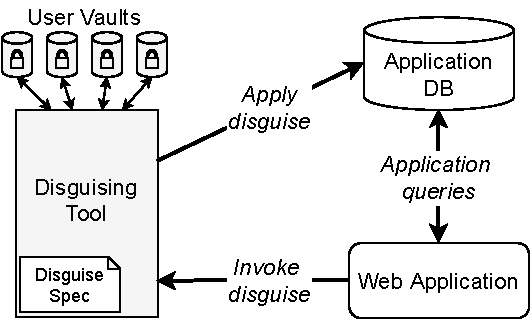
\includegraphics[width=0.5\textwidth]{img/disguise_tool}

    \caption{A data disguising tool sits alongside the application code and database.}
    \label{fig:tool}
\end{figure}


A data disguising tool handles the complexity behind disguise composition, applying disguises in
sequence and generating the necessary storage operations to achieve the correct end state. 
When applying a disguise, the tool must both correctly apply the specified transformations, and also
manage the complexity caused by conflicts and shared dependencies between the new disguise and any
prior disguises.  For example, \texttt{ConfAnon} destroys information linking data records back to a
user, thus making it impossible for \texttt{RTBF} to properly remove these records. 

To handle inter-disguise dependencies, the tool relies on (1) the structured nature of disguises to
statically determine whether disguises share dependencies, and (2) the key abstraction of \emph{user
vaults}, namely per-user logs of disguise updates to that user's data.  User vaults solve the issue
that disguises inherently destroy data necessary to correctly achieve the end-state of future
disguises by providing a secure way to store the data. The tool queries the user vault to
temporarily restore destroyed data (\eg decorrelated foreign key relationships) in order to apply
the disguise correctly.

As shown in Figure~\ref{fig:tool}, a disguising tool sits next to the application, and queries the
user vaults and the application database. The application performs disguises by invoking the tool. 

%-------------------------------------------------------------------------------
\paragraph{Deploying User Vaults.}
%-------------------------------------------------------------------------------
User vaults can be flexibly configured and deployed. It remains important, however, that any
configuration of user vaults should not violate the guarantee that disguises indeed destroy data,
from the viewpoint of the application and any users. 
We imagine several exciting directions to explore for designing vaults that are both
performant and secure.
%

%
Some possible configurations include the tool storing vaults encrypted with a per-user key; this key
may be secret-shared using a (2, 3) threshold scheme~\cite{secretsharing} between the user, the
tool, and a trusted third party (\eg Amazon S3), so that the user can authorize the tool and the
third party to restore the key if the user forgets their share. 
%
The vault entries could be configured to expire after a certain time (requiring that the tool either
prevent future conflicting disguise application, or prevent a-priori disguises that conflict with
legally required disguises such as GDPR deletion). 
%
Or perhaps the vault entries are stored entirely by some third party or locally by the user, whose
server runs a corresponding interface to allow disguise tools to read and write the vault.

The tool should, with user permission, be able to read and write the vaults: a user invoking GDPR
\texttt{RTBF} could provide the key to their vault, and the application invoking the
\texttt{ConfAnon} might notify each user for approval (and temporary vault access) prior to disguise
application. An alternative might be a multi-tier security design, in which the tool and application
are trusted with access to vaults in one tier, allowing them to perform application-instigated
disguises, and untrusted in a second tier, which stores updates from user-invoked disguises.

%\lyt{Might want to say more about how often user vaults are
%queried---what if one disguise needs access to many user vaults, but is being done on behalf of a
%single user? Perhaps there could be multiple ``levels'' of security in vaults, and any
%application-imposed disguise would be protected by application-known keys.}

%-------------------------------------------------------------------------------
\paragraph{Composing and Applying Disguises.}
%-------------------------------------------------------------------------------
Correct composition of multiple disguises achieves an end-state equivalent to combining the
end-states achieved by each disguise when applied to the original application database in isolation.
%
In particular, the tool ensures that prior disguises do not affect \emph{which} objects are updated
by future disguises: a disguise will update all objects that it would have updated if performed on
the original, undisguised state of application data. 

The tool allows developers to reason about multiple conflicting updates to the same object by ensuring that 
if one disguise removes an object that another disguise modifies, the removal takes
precedence.
%
However, if two disguises modify the same object attribute, the tool
establishes no precedence between the modifications and applies them in chronological order.
Alternatively, we can imagine that the developer could specify a partial ordering between
modifications, or restricting the set of possible modifications and establishing a precedence order
within this set.

The tool applies disguises in a four-phase procedure:
\begin{enumerate}
    \item \emph{Prepare}: reconcile any data dependencies between this disguise and prior disguises.
            The tool detects read-after-write dependencies between the new disguise's predicates and prior disguises'
            updates, and, using entries in the vault, undoes any writes that may affect the new disguise's predicates. After
            applying the new disguise updates, the temporarily reversed modifications are reapplied. As an
            optimization, vault entries recording object removals need not be reversed.
        \item \emph{Read}: get all objects that satisfy (per-type) developer-specified predicates.
        \item \emph{Update}: modify, decorrelate, or remove objects read in step (2) according to the
        developer's specification.
    \item \emph{Record}: store records of all updates in the appropriate per-user vaults. The tool
        must be able to determine which user vault should record each modification. This can be
        developer-specified, or rely on a set of heuristics (\eg assigning ownership by traversing,
        starting from each user, the application's object graph expressed in an object-relational
        model (ORM)~\cite{orm}, or implicitly via foreign keys). 
        \lyt{Should we cite Odlaw?}
        %or use techniques such as IFC tracking .  

        \lyt{Should we mention taint tracking/IFC here? We mention in related how
        disguising explicitly does not need such heavyweight techniques.}
\end{enumerate}

%-------------------------------------------------------------------------------
\paragraph{Reversing Disguises.}
%-------------------------------------------------------------------------------
To correctly reverse a disguise and ensure that reintroduced data is not mistakenly revealed because
it missed a subsequent disguise, the tool keeps a persistent log of all disguises performed by the 
application. Any other disguises performed between this disguise's application and its reversal and
applied to any reintroduced data.
